\section{Installationsprozess}\label{sec:installationsprozess}

\subsection{Infrastruktur}

Die ViSIT-Applikationen basieren auf der Server-Client-Architektur. Damit diese Applikationen installiert werden können, wird ein hausinternes Netzwerk (Intranet) und ein damit verbundener Server - lokaler Applikations-Server (kurz LAS) - benötigt. Die ViSIT-Applikationen sind in diesem Zusammenhang die Clients, welche über das Netzwerk mit dem lokalen Applikations-Server verbunden sind. Auf dem LAS ist das ViSIT-System installiert, welches über das Internet Zugang zum globalen ViSIT-Netzwerk hat.
Das ViSIT-System ist eine Ansammlung von mehreren kleinen Applikationen, welche parallel auf dem LAS laufen können. Jeder Client, auf welchem eine der ViSIT-Applikationen läuft, hat eigene Server-Software, welche auf dem LAS installiert ist und für die serverseitigen Berechnungen zuständig ist.

Die Applikationen wurden mit der IT-Technologie “Docker” erstellt. Mit Docker hat man die Möglichkeit, Anwendungen in sogenannten Containern auszuführen und diese Container können aufeinander aufbauen und miteinander kommunizieren. Im Gegensatz zu einer virtuellen Maschine, ist eine Docker-basierte Anwendung nur ein Prozess, der auf dem System ausgeführt wird. Es ist somit kein Gastbetriebssystem erforderlich, wie dies bei Virtuellen Maschinen der Falls ist. Container sind einfach konfigurierbare, abgeschlossene Einheiten, in welchen die Anwendung ausgeführt werden. 
Mit Docker können Linux-Container erstellt und verwendet werden können. Die erstellten Container sind eine Virtualisierung auf der Ebene des Betriebssystems. Durch das Erstellen von Containern, werden isolierte Linux-Systeme auf dem gleichen Host erzeugt. Diese Container können flexibel erstellt, bereitgestellt, kopiert und zwischen Umgebungen verschoben werden. Zweck dieser Container ist die Unabhängigkeit und die Fähigkeit, mehrere Prozesse und Applikationen getrennt voneinander betreiben zu können. Die Vorteile von Docker-Containern sind unter anderem Modularität und Versionsverwaltung. Modularität ermöglicht es, bei zum Beispiel einer Reparatur oder Aktualisierung einer Applikation, nur einen Teil dieser Applikation außer Betrieb zu nehmen, ohne die gesamte Applikation außer Betrieb nehmen zu müssen. Docker bietet eine eingebaute Versionsverwaltung, welche es erlaubt, den aktuellen Stand eines Containers in ein sogenanntes Image zu sichern. Somit ist es möglich, die unterschiedlichen Zustände eines Images in einer Historie nachzuverfolgen. Ein Image ist ein Speicherabbild eines Containers und es besteht aus mehreren Layern, welche schreibgeschützt sind und somit nicht verändert werden können. Ein Layer ist wiederum ein Teil eines Images und enthält einen Befehl oder eine Datei, welche dem Image hinzugefügt wurde. Aufgrund dieser Layer kann die ganze Historie eines Images nachvollzogen werden.

\subsection{Projekt auf dem LAS installieren}

Als erster Schritt muss die Datenbank für die Applikation angelegt werden. Wie oben erklärt, wurde für das ViSIT-Projekt Docker verwendet. Damit gespeicherte Daten auch außerhalb eines Containers abgelegt oder in einem anderen Container eingebunden werden können, werden sogenannte Volumes erstellt. Volumes haben viele Vorteile, vor allem aber sind sie einfacher zu sichern oder zu migrieren. Volumes funktionieren sowohl auf Linux- als auch auf Windows-Containern.
Im ersten Schritt wird ein Volume mit der Datenbank auf dem lokalen Rechner im Terminal mit dem Kommando
\begin{lstlisting}[style=MyBashStyle]
docker volume create visit-database
\end{lstlisting} erstellt. Einen eigenen Volume benötigt man deshalb, weil die dort abgelegten Daten permanent gespeichert werden müssen - würde z.B.: der Container gelöscht oder beendet werden - dann wären die nur im Docker Container gespeicherten Daten ebenfalls gelöscht werden. Damit dies nicht passieren kann, werden die Daten parallel lokal auf dem Rechner gespeichert.
Damit Dateien zwischen Geräten in einem lokalen Netzwerk oder zwischen entfernten Geräten über das Internet synchronisiert werden können, wird eine Datensynchronisation mit Peer-to-Peer-Übertragung benötigt. Dies wird im ViSIT-Projekt mit Syncthing realisiert und auch dafür muss ein eigener Volume lokal auf dem Rechner erstellt werden. Dies geschieht mit \begin{lstlisting}[style=MyBashStyle]
docker volume create visit-syncthing
\end{lstlisting}-Befehl, welcher ebenfalls im Terminal ausgeführt wird.
Als nächster Schritt wird das gesamte ViSIT-Projekt von GitHub mittels

\begin{lstlisting}[style=MyBashStyle]
docker run -d --name visit -p 80:80 -p 22000:22000 -p 21027:21027
-v visit-syncthing:/var/syncthing
-v s:/p2p/visit:/var/p2p
-v visit-database:/var/lib/mysql
--restart unless-stopped visitapp/maincontainer \end{lstlisting}

geklont. Beim erstmaligen Starten benötigt der Vorgang länger, da das Projekt aus dem Git Repository sowie das Appbundle (https://github.com/ViSIT-Dev/appbundle) heruntergeladen werden.\\

Erklärung der einzelnen Befehle:\\
\begin{lstlisting}[style=MyBashStyle]
docker run -d --name visit -p 80:80 -p 22000:22000 -p 21027:21027 
\end{lstlisting}

\begin{lstlisting}[style=MyBashStyle]
docker run 
\end{lstlisting}
 startet den Container und mit den mit den Parametern \begin{lstlisting}[style=MyBashStyle]
-d 
\end{lstlisting} gibt man an, dass der Container im Hintergrund dauerhaft laufen soll (Daemonmode). Weiters wird mit \begin{lstlisting}[style=MyBashStyle]
--name visit
\end{lstlisting} der Name des Containers festgelegt, in diesem Fall heißt der Container visit. Der Container kann im weiteren Verlauf auch über diesen Namen angesprochen werden.
Mit dem Parameter
\begin{lstlisting}[style=MyBashStyle]
-p 80:80
\end{lstlisting} werden die Ports vom Host an den Container gebunden. Hier wird der lokale Hostport 80 auf den Containerport 80 gemappt. Die weiteren Ports 
\begin{lstlisting}[style=MyBashStyle]
-p 22000:22000 -p 21027:21027 
\end{lstlisting} werden für das Syncthing und für das Peer to Peer-Netzwerk benötigt.
Als nächstes folgt der Befehl 
\begin{lstlisting}[style=MyBashStyle]
-v visit-syncthing:/var/syncthing
\end{lstlisting}
Mit dem Parameter \begin{lstlisting}[style=MyBashStyle]
-v
\end{lstlisting}
 wird ein Verzeichnis (Volume) auf dem Hostrechner zu einem Verzeichnis innerhalb des Containers verbunden, auf diese Weise werden die Daten persistent gespeichert, das heißt, dass ein Ordner auf dem Hostsystem auf einen Ordner im Container gemappt wird. Das bedeutet, dass die Daten in beiden Ordnern immer inhaltsgleich sind. Ohne dem Mapping zu einen Ordner auf dem Hostsystem, wären alle Daten aus dem Docker Container, wenn dieser Container gelöscht wird, ebenfalls gelöscht. Um die Daten persistent, also dauerhaft zu speichern, wird immer ein Ordner im Hostsystem mit dem entsprechenden Ordner im Docker Container gemappt.
Zuerst wird das Verzeichnis auf dem Hostrechner angegeben, hier \begin{lstlisting}[style=MyBashStyle]
visit-syncthing
\end{lstlisting}
und nach dem Doppelpunkt steht das Verzeichnis innerhalb des Containers, hier \begin{lstlisting}[style=MyBashStyle]
/var/syncthing
\end{lstlisting}

Im nächsten Teil des Befehls \begin{lstlisting}[style=MyBashStyle]
-v s:/p2p/visit:/var/p2p
\end{lstlisting}
 wird ebenfalls zuerst das Verzeichnis auf dem Hostrechner angegeben, \begin{lstlisting}[style=MyBashStyle]
s:/p2p/visit
\end{lstlisting} und dann das Verzeichnis innerhalb des Containers \begin{lstlisting}[style=MyBashStyle]
/var/p2p
\end{lstlisting}
Im nächsten Befehl \begin{lstlisting}[style=MyBashStyle]
-v visit-database:/var/lib/mysql
\end{lstlisting} geht es um die Verbindung zur Datenbank. Hier wird ebenfalls zuerst das Verzeichnis auf dem Hostrechner angegeben \begin{lstlisting}[style=MyBashStyle]
visit-database
\end{lstlisting} und nach dem Doppelpunkt steht das Verzeichnis innerhalb des Containers \begin{lstlisting}[style=MyBashStyle]
/var/lib/mysql
\end{lstlisting}
Zuletzt wird mittels \begin{lstlisting}[style=MyBashStyle]
--restart unless-stopped visitapp/maincontainer
\end{lstlisting} dem System mitgeteilt, dass der Docker Container \begin{lstlisting}[style=MyBashStyle]
visitapp/maincontainer
\end{lstlisting} automatisch gestartet werden soll außer, wenn er manuell oder anderweitig gestoppt wird.

Wenn der Vorgang abgeschlossen ist, kann über Lokalhost im Browser unter \textbf{localhost:80/typo3/} das Backend aufgegerufen werden. Das erstmalige einloggen in das Backend (TYPO3) erfolgt mit dem \textbf{Benutzername: admin} und \textbf{Passwort: visit-admin}.

\begin{figure}[ht!]
\centering
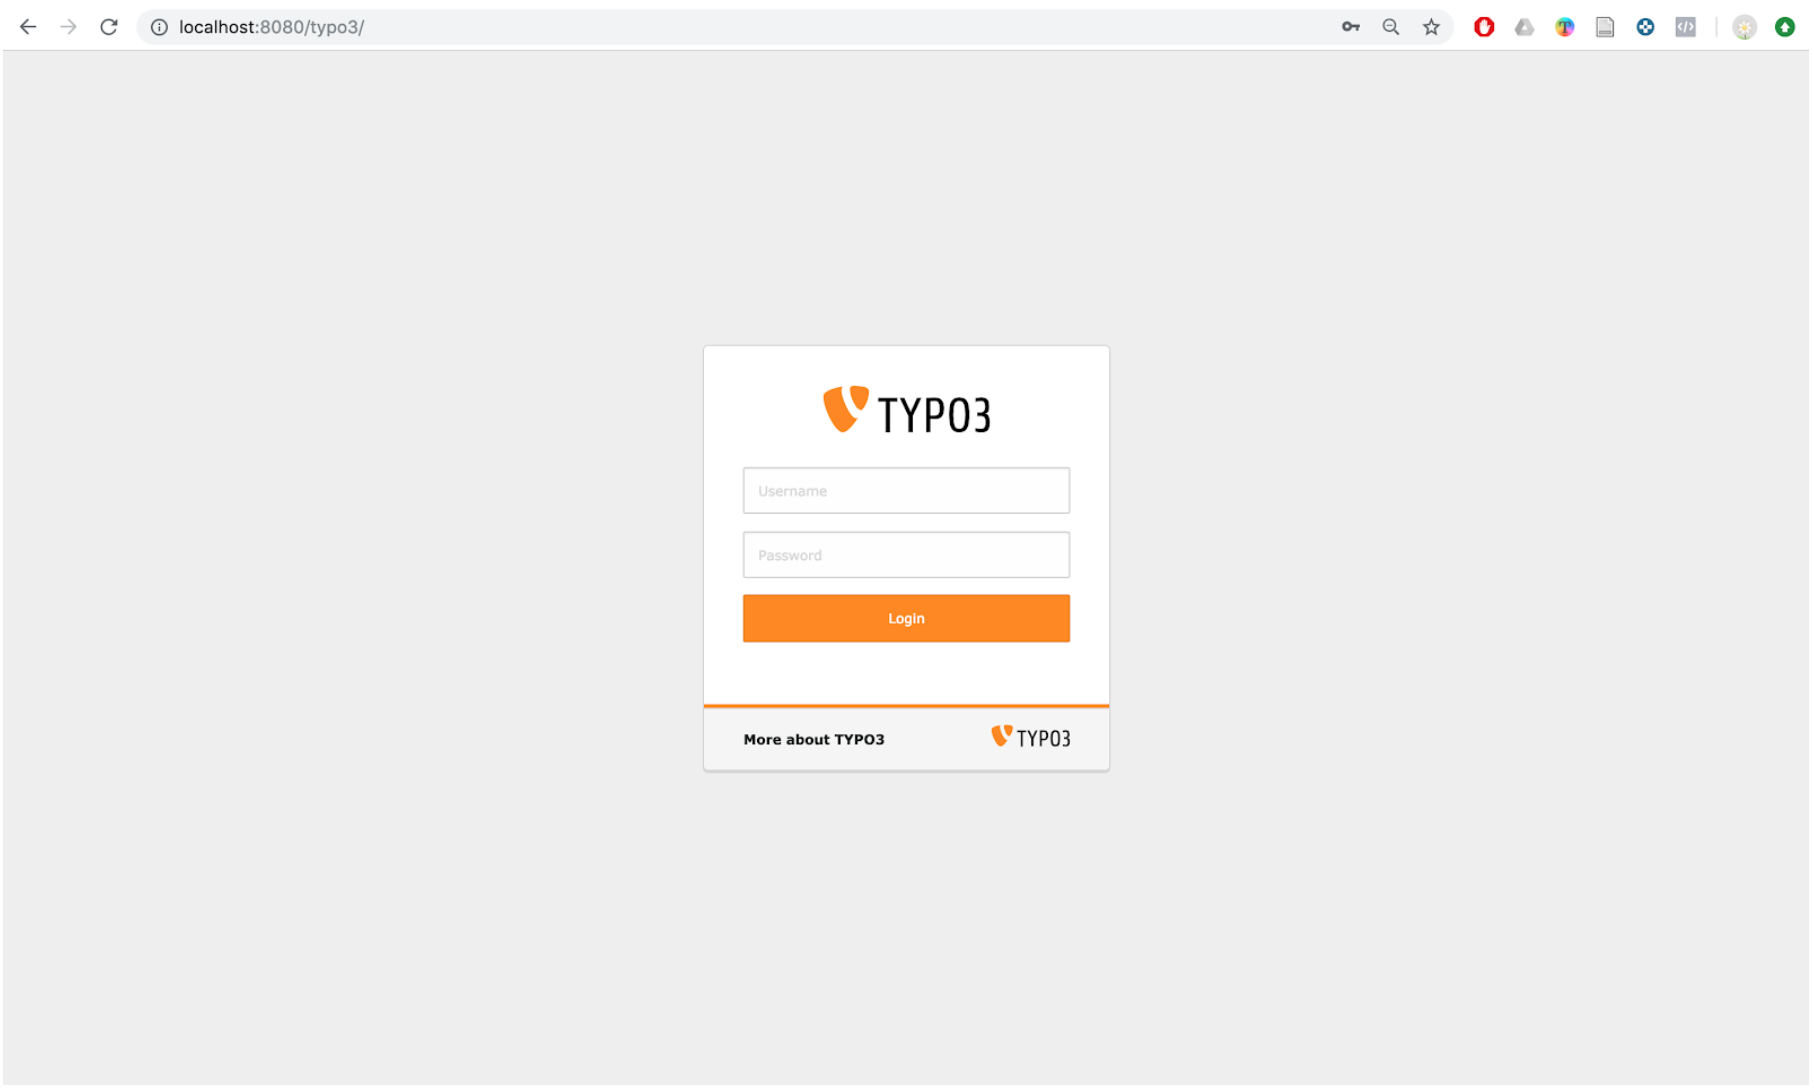
\includegraphics[width=12cm]{Figures/paula/typo_3_login.png}
\caption{Das Login-Fenster für TYPO3}
\label{img:typo_3_login}
\end{figure}

\section{TYPO3}
\subsection{Allgemein}

TYPO3 ist ein freies Content-Management-System für Webseiten, es wird in Frontend und Backend getrennt. Als Frontend wird die Präsentationsebene bezeichnet, das ist der Teil einer Applikation, den der Betrachter sehen kann. Als Backend hingegen, bezeichnet man die Datenzugriffsebene, das ist der Teil einer Applikation, welcher nicht für den Besucher sichtbar ist. Das Backend ist der Verwaltungsbereich einer Webseite. TYPO3 wird auf einem Webserver installiert und über den Webbrowser benutzt.
Das Backend kann man sich als eine Werkstatt vorstellen in der Sachen produziert und gelagert werden und wenn sie fertig sind, ins Schaufenster, dem Frontend, gestellt werden und von Besuchern bestaunt werden können.

\subsection{Login}

Damit niemand unbefugter im Frontend sowie Backend etwas verändern kann, muss man sich zuerst ins Backend einloggen. Dies geschieht über den Aufruf der Domain \textbf{localhost:80/typo3/} im Webbrowser.

\begin{figure}[ht!]
\centering
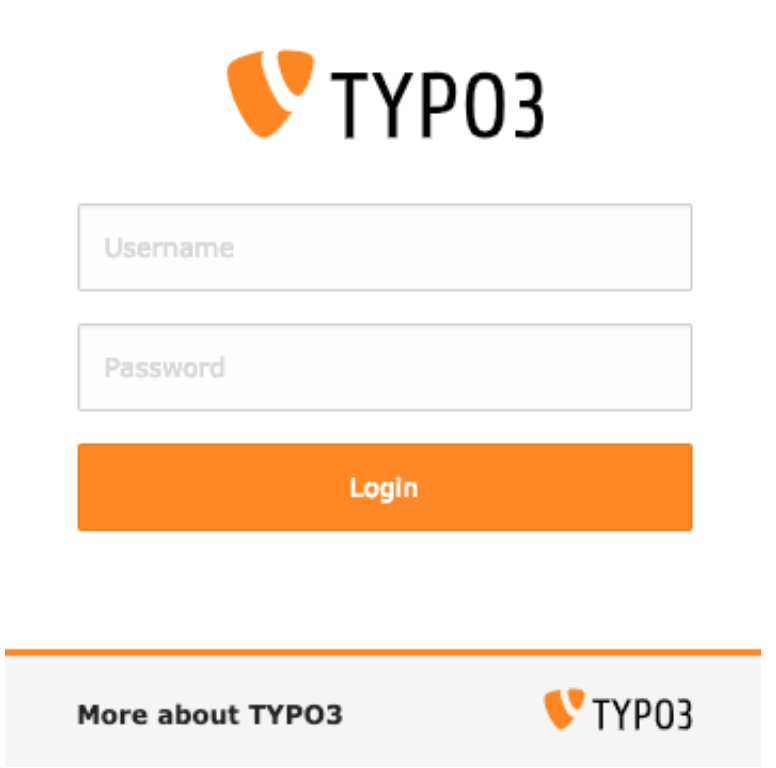
\includegraphics[width=12cm]{Figures/paula/login_TYPO3.png}
\caption{Das Login-Fenster für TYPO3}
\label{img:typo_3_logIn}
\end{figure}

Im Login-Fenster kann der Benutzername sowie das Passwort eingetragen werden. Beim ersten Login ist der \textbf{Benutzername: admin} und das \textbf{Passwort: visit-admin}, dieser muss in weiterer Folge verändert werden. Mehr dazu siehe Anpassung.
Nach einem erfolgreichen Login wird das Backend mit den dazugehörigen Modulen im Browser geladen.

\begin{figure}[ht!]
\centering
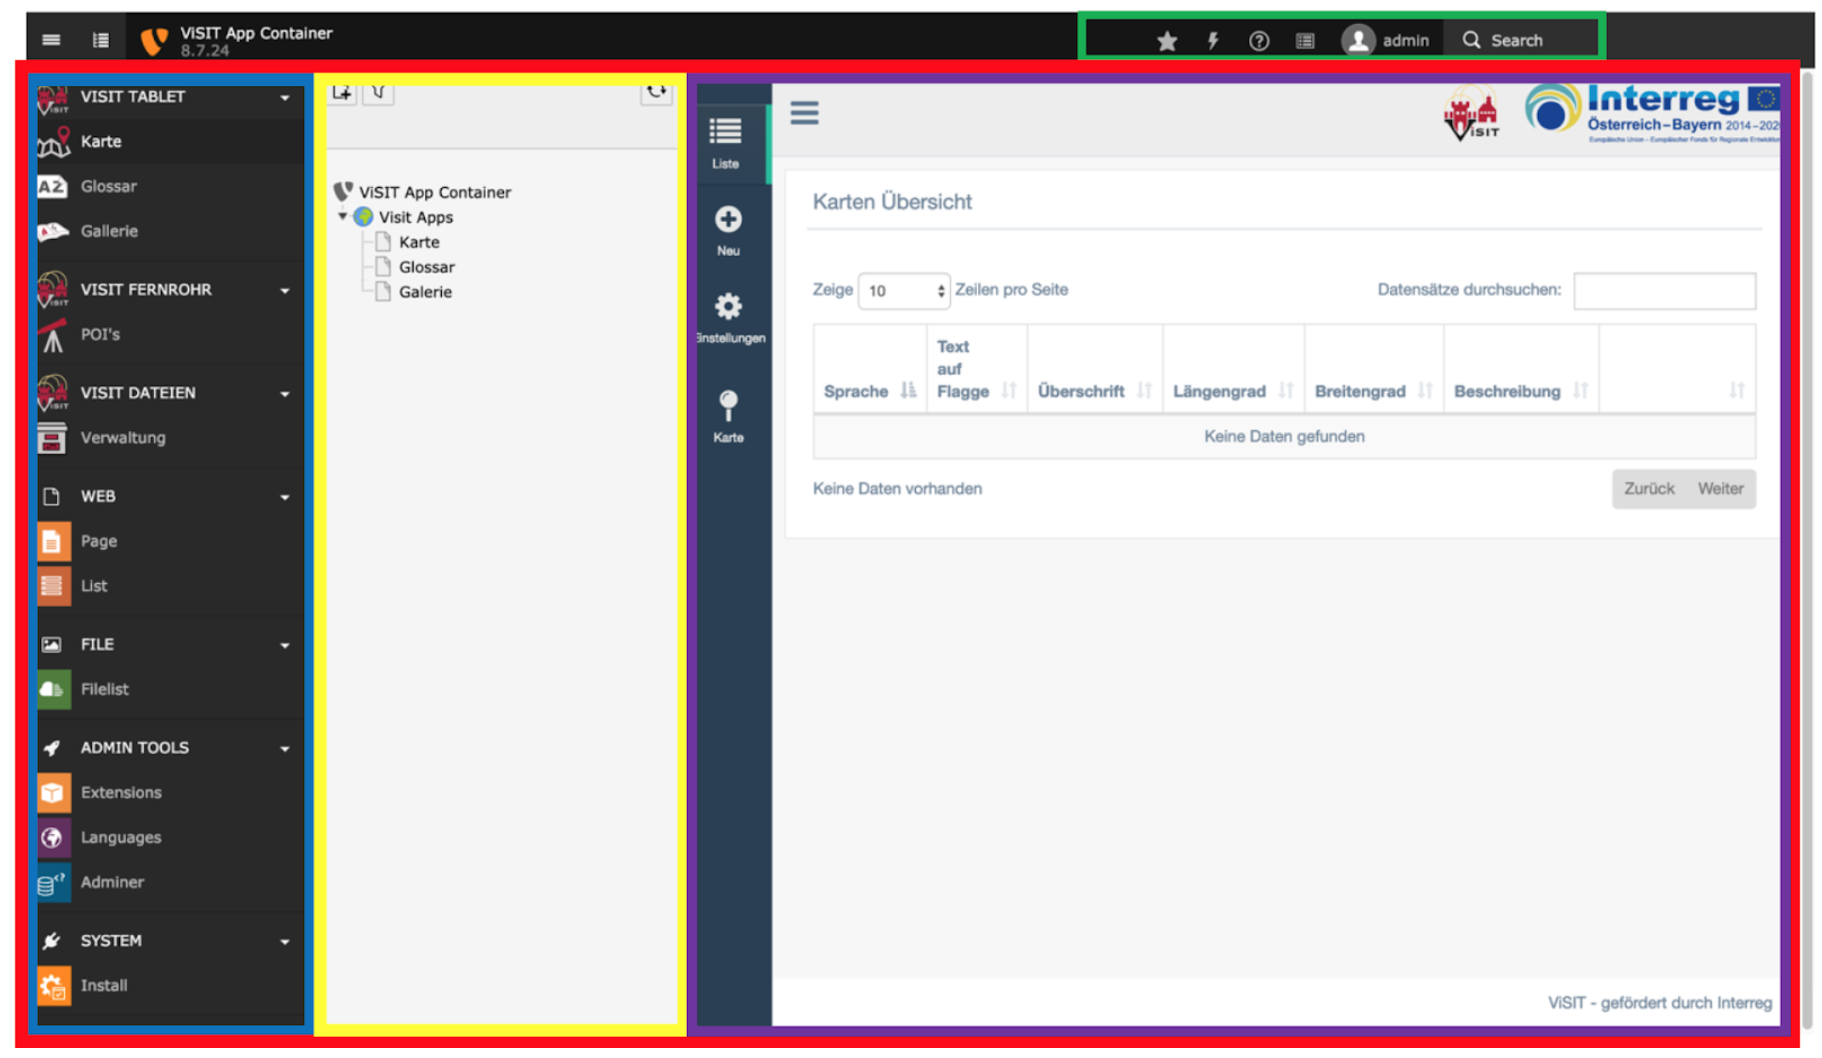
\includegraphics[width=12cm]{Figures/paula/aufbau_TYPO3.png}
\caption{Aufbau des TYPO3-Backends}
\label{img:typo_3_backend}
\end{figure}

\subsection{Aufbau von TYPO3}

Das TYPO3-Backend besteht aus einem Kopfbereich (grün eingerahmt) und einem Hauptbereich (rot eingerahmt), welcher aus drei Spalten besteht. Im Kopfbereich kann der Administrator seine TYPO3-Benutzerenstellungen konfigurieren. Im Hauptbereich werden Webdokumente bearbeitet. Das TYPO3-Backend wird von links nach rechts abgearbeitet.


\cite{anno4j1}